\subsection{Experiments}
\label{subsec:experiments}

The training procedure is illustrated in Figure~\ref{fig:training-overview}. We train our model on a dataset of paired digital-film images. As our image dataset is relatively small, we use a patched training approach, where we randomly sample patches of size $256 \times 256$ from the images before feeding them into the model. We train our model on 400 patches per image in the dataset using the Adam optimizer with a learning rate of $1e-3$ and a batch size of 1. Our experiments are divided into two parts: single-image experiments and full dataset experiments.

\begin{figure}
  \centering
  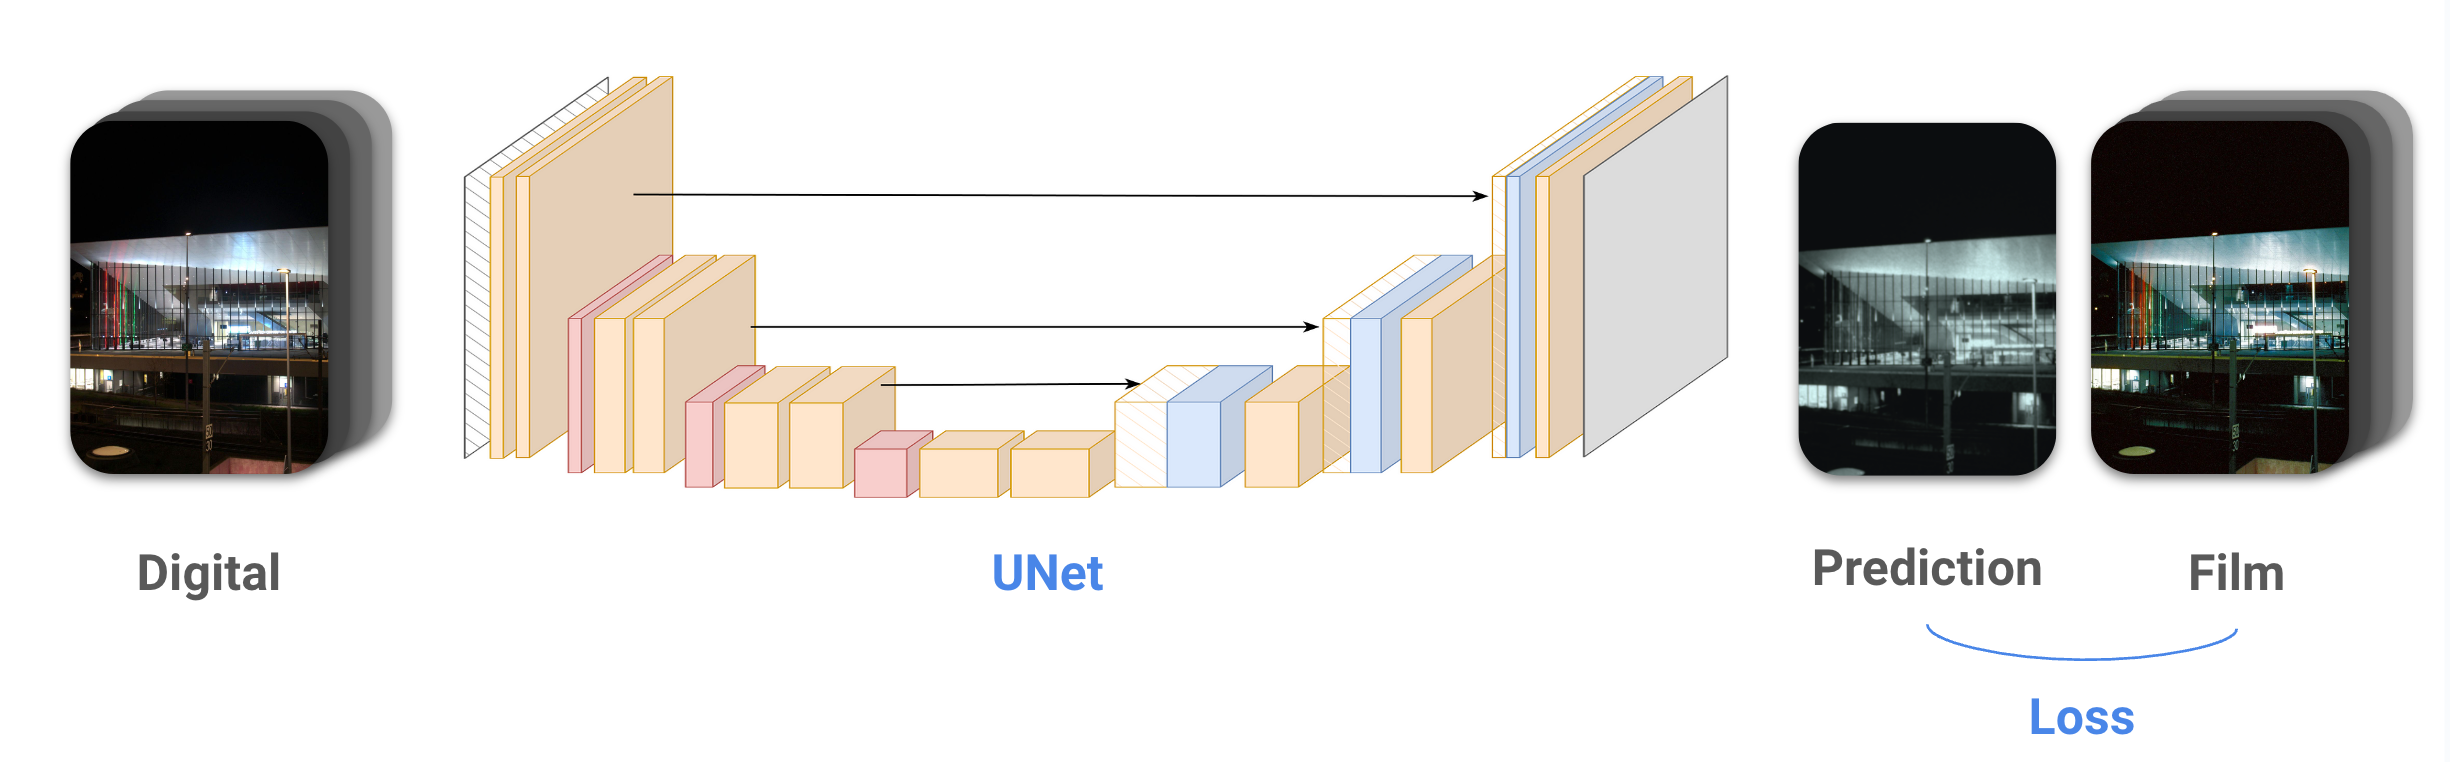
\includegraphics[width=0.9\textwidth]{figures/training-overview.png}
  \caption{\textbf{Training Overview.} We train our model on paired digital-film images.}
  \label{fig:training-overview}
\end{figure}

% Single image experiments
For our single-image experiments, we handpicked an image from our dataset that contains a white wall with a light source. It was chosen for the clear blue tint of the film effect and the clearly perceptible grain on the uniform background. For these experiments, we train and evaluate the model on the same image. We first investigate how each loss produces the desired colour effect to gain a better understanding of the interplay between the loss functions and what the model learns.

% Full dataset experiments
For the most promising candidates from the single-image experiments, we then
move on to training on the full dataset. The full dataset is split into a
training, validation and test set using a 70-20-10 split ratio, but final evaluation is done on the full dataset.

% Adding noise channel and resizing
We also investigate whether adding noise as a 4th input channel to the model improves the its ability to learn the desired visual effects for both single image and full dataset experiments. This is done by concatenating a random uniform noise \footnote{We tried using other forms of noise such as Guassian noise but found that this made little difference.} channel to the input images.  Furthermore, we observed that patched training is very stochastic as each patch only captures a very small portion of the original image and can be very different from the rest of the image. To contain more information in each patch we also experiment applying a resized crop where we first crop the image to a larger patch and then resize to the desired input size. This way we can ensure that each patch contains more information from the original image.

